\chapter{Implementation}
The implementation of the project began on schedule at the beginning of week 2. The following chapter describes how the design was implemented in the development of a working system. Important code samples and functions have been included where appropriate. Using the chosen methodology, development ran in a series of iterations, at the end of each the different parts of the system were expected to work.

For the system development it was required to have access to the PTU to test the code functionality. The PTU was unmounted from the rover, brought to the Digital Systems Laboratory and connected to the power supply.

Replacement of the Gumstix to the Raspberry Pi minicomputer and all the necessary wiring was done by the laboratory technician who I am very grateful to. Otherwise it would probably have taken a few more weeks of my time to find out how everything should be fitted in. 

\section{Iteration 0}
Current system porting
excellent documentation about GPIO14

\section{Iteration 1}
TASS library new commands
 
\section{Iteration 2}
PTU TASS library improvement
\subsection{Stabilise command}
\label{stabilize_implementation}
 This is a relatively simple task since it just requires for the two digits to be added to the final message and sent to the PTU. However before doing this project I didn't know much about the ASCII table. I ended up spending a significant amount of time reading and rereading PTU documentation ~\ref{fig:pushDfunction}
 
 \begin{figure}[H]
 \centering
 \centerline{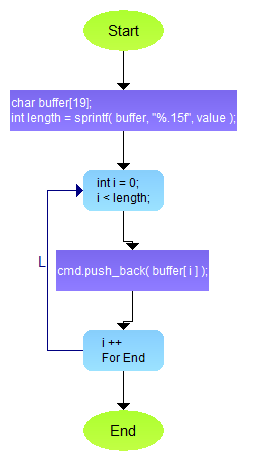
\includegraphics[scale=0.65]{./images/pushDfunction}}
 \caption{Flow for the function to translate doubles in to the ASCII encoding}
 \label{fig:pushDfunction}
 \end{figure}
 
 
 \section{Stabilization with drift compensation}
 
 The algorithm presented below will work only if we assume that vertical position of the PTU platform is desired. It does not accommodate the case when the PTU  platform is stabilized at the position other that vertical. This was found at the time of writing report and could be fixed given the more time.
 
 \section{AberBox \& AberBox API improvements}
